\documentclass[UTF8,a4paper,zihao=5,fontset=windows]{ctexart}
\usepackage[margin=22mm,headheight=15pt]{geometry}
\usepackage{amsmath,amssymb,bm,mathtools}
\usepackage{booktabs,longtable,tabularx,array,graphicx,xcolor}
\usepackage{caption,enumitem,fancyhdr,hyperref,placeins}
\definecolor{navy}{HTML}{174766}
\hypersetup{colorlinks=true,linkcolor=navy,citecolor=navy,urlcolor=navy,
 pdftitle={八线圈磁驱动与进退镜视觉协同：胶囊机器人导航的方法论与单例仿真},
 pdfauthor={项目方法整理},pdfsubject={动力学、磁场优先分配、摄像头规划与闭环边界}}
\graphicspath{{../figures/}}
\pagestyle{fancy}\fancyhf{}
\fancyhead[L]{\small 八线圈磁驱动与进退镜视觉协同}
\fancyhead[R]{\small 方法论与单例仿真}
\fancyfoot[C]{\thepage}
\setlength{\parindent}{2em}\setlength{\parskip}{3pt}
\setlength{\emergencystretch}{2em}\linespread{1.14}
\renewcommand{\arraystretch}{1.22}
\captionsetup{font=small,labelfont=bf,skip=6pt}
\setlist{nosep,leftmargin=2em}\numberwithin{equation}{section}
\setcounter{tocdepth}{1}
\makeatletter\setlength{\@fptop}{0pt}\makeatother
\newcommand{\vect}[1]{\bm{#1}}
\newcommand{\norm}[1]{\left\lVert#1\right\rVert}
\newcommand{\clip}{\operatorname{clip}}
\newcommand{\sat}{\operatorname{sat}}
\newcommand{\wrap}{\operatorname{wrap}}
\newcommand{\diag}{\operatorname{diag}}
\newcommand{\tr}{\operatorname{tr}}
\newcommand{\dd}{\mathrm{d}}
\newcommand{\unit}[1]{\,\mathrm{#1}}
\newcommand{\code}[1]{\texttt{\detokenize{#1}}}
\newenvironment{boundary}{\begin{quote}\small\color{navy}\textbf{适用边界。}}{\end{quote}}
\title{\heiti 八线圈磁驱动与进退镜视觉协同：\\胶囊机器人导航的方法论与单例仿真}
\author{现有项目实现的可追溯方法稿}
\date{2026年10月18日}
\begin{document}
\maketitle\vspace{-1em}
\begin{center}\small 基于 clon001 当前有效实现；非有限元、实物线圈或临床验证报告\end{center}
\begin{abstract}
针对结肠胶囊机器人沿既定路线运动与内壁观察难以同时协调的问题，本文整理一种由空间路径反馈、磁场优先电流分配、刚体动力学和进退镜摄像头规划组成的方法。胶囊不按预设时间表直接更新位置，而由八个受电流约束的等效线圈磁源产生合成磁场和梯度，经磁力、磁转矩及理想滑动阻力驱动。控制器优先满足长轴调向所需磁场，再利用磁场映射的零空间补足推进力；八磁源相对布局固定，仅整体限速平移。进镜摄像头继承随弧长索引的前瞻目标，并依据实际机身姿态执行受限比例微分控制；退镜在前向锥内进行粗细两级密集视场搜索，预测未来1.2秒的去重观察收益，在收益接近最优的可行方案中优先选择平滑运动。相机误差和角速度降低导航速度上限，不设相机停车等待。本文给出动力学、磁源叠加、优先级分配、可见性、观察时长及局部闭环稳定性条件。单一 clon001 几何上，进退镜分别用时294.84秒和303.70秒，最大单路电流约9.19安培；几何有效覆盖由67.17\%增加至79.85\%。这些结果仅支持所选参数与同一模型下的数值可行性，不证明硬件可实现性、全局闭环稳定性或临床诊断获益。方法的潜在价值在于将磁驱动约束、镜头连续运动和退镜补充观察放入同一可检验流程，为后续传感闭环、线圈标定和体模研究提供接口。
\end{abstract}
\noindent\textbf{关键词：}磁驱动胶囊机器人；八线圈阵列；磁场优先；路径跟随；主动视觉；短时预测；几何观察覆盖
\begin{quote}\small
\textbf{English abstract.} This implementation-grounded methods study combines spatial path feedback, field-priority current allocation, rigid-body dynamics, and insertion/withdrawal camera planning for a magnetic capsule. Eight current-bounded point-dipole sources generate the applied field and gradient; capsule poses are integrated rather than prescribed by a replay clock. Insertion reuses arc-indexed look-ahead targets, whereas withdrawal uses coarse-to-fine view search and a 1.2-s prediction horizon to favor smooth, near-best coverage gains. Camera tracking difficulty reduces the navigation speed envelope without a camera-wait command. A single clon001 simulation completed insertion and withdrawal in 294.84 and 303.70 s. The peak current was 9.19 A and geometric observation coverage increased from 67.17\% to 79.85\%. These results establish internal numerical feasibility only. Hardware field calibration, contact mechanics, sensing, global stability, and clinical benefit remain unverified.
\end{quote}
\clearpage\tableofcontents\clearpage

\section{研究问题、文献依据与贡献边界}
\subsection{研究目标}
本文研究的问题是：在已知三维结肠内表面和既定进镜路线的条件下，能否用受限的外部磁源输出使胶囊完成“肛门入口、肠道深部、同一肛门入口”的往返，同时保持摄像头运动连续，并在退镜时补充进镜未充分观察的区域？目标不是逐时刻复现旧轨迹，也不是以高播放帧率代替真实动力学。

以路线几何为参考，胶囊的位移和姿态由运动方程决定。风险、净空、曲率和相机运动难度参与调节导航速度上限；机器人可推进或制动，但不加入等待镜头的状态机。观察效果用有遮挡和观察时长门槛的面片面积衡量，不将画面中出现过的所有区域直接计为已检查。

\subsection{相关工作的作用与差异}
Kummer等提出的OctoMag系统是多线圈磁操纵的代表性工作\cite{kummer2010}。该文为多源场与梯度控制提供背景，但本文的阵列布局、磁源系数和工作空间不能视为对OctoMag硬件的复现。Cai等研究了磁场优先的可重构电磁操纵\cite{cai2025}：三个线圈分别搭载于独立机械臂，通过电流满足磁场要求，并通过线圈位姿多目标优化改善磁力，同时考虑机械臂可操作度。本文借鉴的是“先满足磁场，再改善磁力”的控制顺序。

当前实现与上述三机械臂系统有实质区别：采用八个相对固定的等效源，利用电流冗余求解磁力，仅使阵列整体平移随行；没有逐线圈位姿搜索、机械臂逆运动学、可操作度优化或碰撞求解。因此，文献中“三个可独立重配置线圈可行”，与本文所选受限布局下“八源案例跑通”，并不矛盾。本文也不由本例推断七源一定失败、九源一定无效，或八源具有普遍最小性。

Martin等将机器人、视觉与控制结合，用于磁性内镜的智能和自主操纵\cite{martin2020}，说明运动控制与视觉任务协同具有研究依据；但本项目并未复现其视觉定位或活体实验。本文的反馈状态直接来自仿真，观察评价依赖已知网格，不是临床内镜视频闭环。

\subsection{四个方法模块}
四个模块分别为：机器人平移与长轴姿态的动力学解算；八等效线圈的空间磁场、梯度与电流分配；进镜前瞻摄像头目标及关节控制；退镜密集搜索、短时预测和补充覆盖。它们通过实际状态、相机误差、速度上限和覆盖记忆相互连接，结构见图\ref{fig:architecture}。
\begin{figure}[htbp]
\centering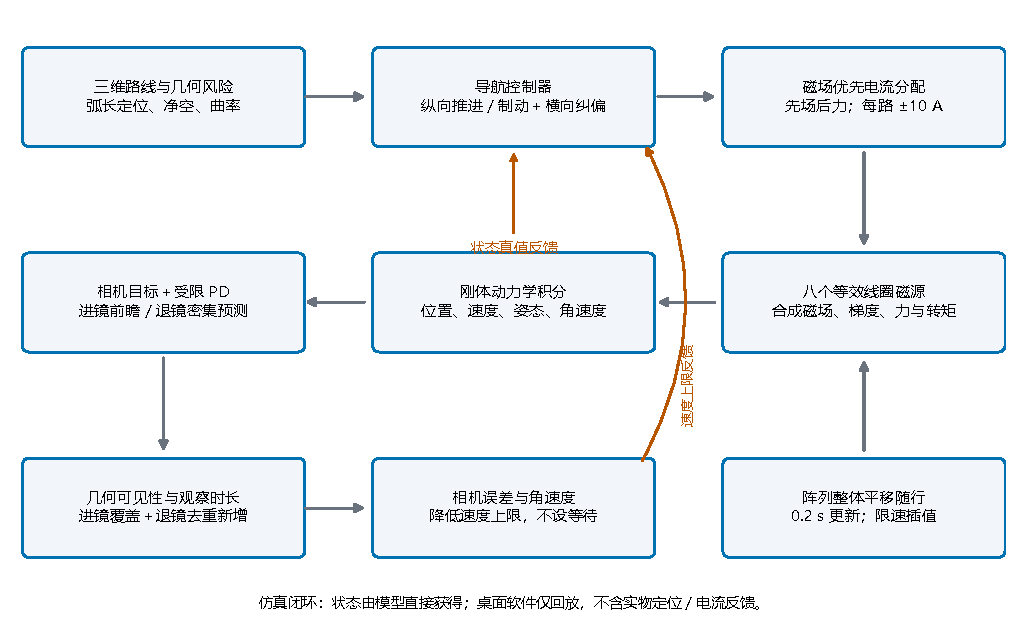
\includegraphics[width=\linewidth]{fig01_architecture.pdf}
\caption{现有实现的反馈结构。橙色表示状态或速度上限反馈。场与梯度由同一磁源模型计算，状态由模型直接获得。阵列只整体平移，反馈箭头不代表已经实现实物定位或电流传感闭环。}\label{fig:architecture}
\end{figure}

\section{几何、坐标与建模假设}
\subsection{路线、体位与进退镜方向}
记世界坐标系为$\mathcal W$，世界$+Z$竖直向上。原始网格经共同刚体变换置于仰卧展示姿态：
\begin{equation}
\vect p^{\mathcal W}=R_S\vect p^{\rm raw}+\vect t_S,
\quad R_S=\begin{bmatrix}1&0&0\\0&0&-1\\0&1&0\end{bmatrix},
\quad \vect g^{\mathcal W}=\begin{bmatrix}0&0&-9.81\end{bmatrix}^{\mathsf T}\unit{m/s^2}.
\label{eq:supine}
\end{equation}
网格、路线、法向和参考机身姿态同步变换，重力始终固定于世界$-Z$，不是将旧重力与网格一起旋转。平移量为$(-17.4710,-316.4328,306.9087)^{\mathsf T}$毫米。原始网格的解剖方向未经患者配准核验，故这里是体位假设，不是对患者真实仰卧解剖的恢复。

用全局弧长$s\in[0,L]$标记路线，$s=0$固定对应肛门，$L=1722.3136\unit{mm}$对应深部。进镜时$s$增加；退镜在代码内部使用局部弧长$\sigma=L-s$增加。换向不要求胶囊掉头，参考长轴仍继承原路线姿态，因此退镜可以表现为沿胶囊长轴反向移动。两阶段传递实际位置、速度、四元数、角速度、云台状态和阵列锚点，不将它们重置到参考值。

横卧坐标中的肛门入口为$(-16.5008,189.8172,161.3417)$毫米，深部为$(18.0622,25.7672,49.7367)$毫米。完成条件同时检查剩余局部弧长不超过$0.15\unit{mm}$和距阶段终点不超过$1\unit{mm}$，不通过位置吸附达成终点。图\ref{fig:geometry}给出路线与初始源位置。
\begin{figure}[htbp]
\centering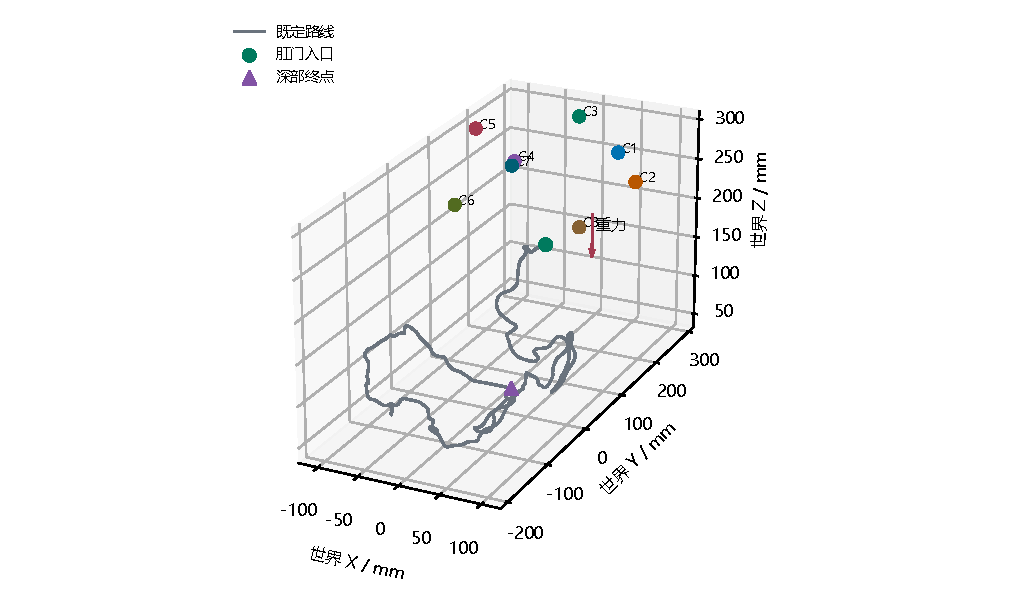
\includegraphics[width=.92\linewidth]{fig02_geometry.pdf}
\caption{仰卧摆放假设下的路线、重力和初始八磁源位置。各坐标轴以毫米计，三维盒比例按坐标跨度设置。C1--C8为点磁源标记，不表示线圈真实半径、绕组或铁芯形状。阵列位于锚点世界$+Z$一侧不等于已验证其与整个患者体表无碰撞。}\label{fig:geometry}
\end{figure}

\subsection{胶囊尺寸、质量、磁矩与惯量}
胶囊按长$\ell=12\unit{mm}$、直径$d=6\unit{mm}$建模。质量和磁矩由既有参考参数按体积比例缩放：
\begin{equation}
\eta=\frac{12}{25}\left(\frac{6}{13}\right)^2=0.1022485,
\quad M=0.00516\eta=5.2760\times10^{-4}\unit{kg},
\quad m_0=0.253\eta=0.0258689\unit{A\,m^2}.
\label{eq:scaling}
\end{equation}
这是项目继承的工程假设，不是称重或磁矩实测。外观虽绘成胶囊，动力学惯量按均匀椭球估计。设半轴$a=\ell/2$、$b=c=d/2$，则
\begin{equation}
J=\frac{M}{5}\diag(b^2+c^2,a^2+c^2,a^2+b^2)
=\diag(2.1843,5.7456,5.7456)\times10^{-9}\unit{kg\,m^2}.
\label{eq:inertia}
\end{equation}
机身旋转矩阵$R$将机体系向量映射到世界系。机身$+X$为胶囊长轴，单位方向$\vect u=R\vect e_1$，胶囊磁矩为$\vect m=m_0\vect u$。单一固定磁偶极不能直接产生沿$\vect m$方向的转矩，因而长轴指向可控并不意味着机身三轴姿态均独立可控。

\subsection{假设层级}
当前采用静态已知网格、刚性胶囊、磁准静态线性叠加、理想电流执行与简化滑动阻力。八源位置和状态均已知，无定位噪声或通信延迟。没有肠壁弹性、接触反力、蠕动、浮力、流体、真实照明、组织纹理或病灶识别模型。路线点处净空可出现零值；“数值走完”不能据此证明有限尺寸胶囊无接触穿行。本文将这些假设作为结果成立的条件，而非用覆盖率或小跟踪误差替代安全验证。

\section{机器人动力学与理想磁需求}
\subsection{平移、转动与四元数积分}
状态取$\vect x=(\vect p,\vect v,\vect q,\vect\omega_b)$，其中四元数按$(q_x,q_y,q_z,q_w)$排列，$\vect\omega_b$为机体系角速度。平移满足
\begin{equation}
\dot{\vect p}=\vect v,\qquad M\dot{\vect v}=\vect F_{\rm mag}+\vect F_{\rm fr}+M\vect g.
\label{eq:translation}
\end{equation}
理想摩擦/滑动阻力沿用现有公式：
\begin{equation}
N_{\rm eff}=M\norm{\vect g},\qquad
\vect F_{\rm fr}=-\mu N_{\rm eff}\frac{\vect v}{\sqrt{\norm{\vect v}^2+v_\epsilon^2}},
\quad\mu=0.2,\quad v_\epsilon=0.5\unit{mm/s}.
\label{eq:friction}
\end{equation}
它在零速附近平滑，高速时接近固定幅值滑动阻力；$N_{\rm eff}$不是求解出的肠壁法向接触力，也没有静摩擦粘滞区。因此，当前不模拟静摩擦导致的卡住、黏液润滑变化或真实接触压力。

转动及四元数演化为
\begin{align}
J\dot{\vect\omega}_b+\vect\omega_b\times(J\vect\omega_b)&=R^{\mathsf T}\vect\tau_{\rm mag},\label{eq:rotation}\\
\dot{\vect q}_v&=\tfrac12(q_w\vect\omega_b+\vect q_v\times\vect\omega_b),\qquad \dot q_w=-\tfrac12\vect q_v^{\mathsf T}\vect\omega_b.
\label{eq:quaternion}
\end{align}
每个动力学步后将四元数归一化。真实施加于式\eqref{eq:translation}和\eqref{eq:rotation}的量来自八源输出，而不是直接用理想需求替换磁力和磁转矩。

\subsection{力、转矩与局部磁场关系}
定义$G_{jk}=\partial B_j/\partial x_k$，当胶囊磁矩在局部空间求导中视为固定时，
\begin{equation}
\vect F_{\rm mag}=G^{\mathsf T}\vect m,\qquad \vect\tau_{\rm mag}=\vect m\times\vect B.
\label{eq:wrench}
\end{equation}
在不含源电流、磁导率均匀的局部区域，磁准静态模型满足
\begin{equation}
\nabla\cdot\vect B=0,\quad \nabla\times\vect B=0,\qquad \tr G=0,\quad G=G^{\mathsf T}.
\label{eq:maxwell}
\end{equation}
这些约束不能直接用于铁芯内部、导线位置或材料界面。点偶极场在源位置本身具有奇点。

\subsection{理想反解是需求接口，不是磁源实现}
给定期望转矩$\vect\tau_c$，先去除单偶极无法支持的轴向分量：
\begin{equation}
\vect\tau_\parallel=(\vect\tau_c\cdot\vect u)\vect u,\quad
\vect\tau_\perp=\vect\tau_c-\vect\tau_\parallel,\quad
\vect B_d=\frac{\vect\tau_\perp\times\vect m}{m_0^2}+B_0\vect u,\quad B_0=0.01\unit T.
\label{eq:field_inverse}
\end{equation}
于是$\vect m\times\vect B_d=\vect\tau_\perp$，而平行偏置项本身不对当前磁矩产生转矩。10毫特斯拉是当前选定的偏置幅值，不是每个线圈各有10毫特斯拉，也不是经实验优化的临床参数。

若仅求满足理想力$\vect F_c$的最小Frobenius范数、对称无迹梯度，记
\begin{equation}
\alpha=\frac{\vect F_c\cdot\vect u}{m_0},\qquad
\vect\beta=\frac{\vect F_c-(\vect F_c\cdot\vect u)\vect u}{m_0},
\end{equation}
则既有理想解为
\begin{equation}
G_{\rm ideal}=\alpha\left(\tfrac32\vect u\vect u^{\mathsf T}-\tfrac12 I_3\right)
+\vect\beta\vect u^{\mathsf T}+\vect u\vect\beta^{\mathsf T}.
\label{eq:ideal_gradient}
\end{equation}
该式满足$G_{\rm ideal}^{\mathsf T}\vect m=\vect F_c$和式\eqref{eq:maxwell}的局部约束，但并不保证某个真实阵列能产生它。在当前八源系统中，它仅用于理想参考与导出对照；电流分配直接匹配场和力，\textbf{没有强制实际梯度矩阵逐元素等于$G_{\rm ideal}$}。
\section{空间路径反馈、风险地图与只减速协调}
\subsection{空间参考与局部投影}
路线位置$\vect r(\sigma)$由三次样条表示，参考姿态$R_r(\sigma)$由弧长节点旋转插值表示，单位切向为$\vect t=\vect r'/\norm{\vect r'}$。当前代码使用局部折线投影估计弧长，而在该弧长处查询样条参考；两者差异属于离散近似，不把样条参考点强行写回实际位置。

对折线段$[\vect r_j,\vect r_{j+1}]$，计算
\begin{equation}
\lambda_j=\clip\!\left(\frac{(\vect p-\vect r_j)^{\mathsf T}(\vect r_{j+1}-\vect r_j)}{\norm{\vect r_{j+1}-\vect r_j}^2},0,1\right),\quad
\hat{\vect p}_j=\vect r_j+\lambda_j(\vect r_{j+1}-\vect r_j).
\label{eq:projection}
\end{equation}
在上次弧长附近$\pm25\unit{mm}$的窗口中选择最近投影，并相应限制段内参数。该局部约束减少空间相邻但弧长相隔很远的肠袢之间跳段的风险，但不构成有噪声定位下的全局匹配保证。

\subsection{几何风险输入与速度上限}
当前导航复用已生成的几何风险和三类速度上限，而不在每次积分中重建风险地图。上游路径代价包括贴壁、狭窄、曲率、敏感区及运动代理项。对半径$\rho$（毫米）、转向角$\psi$和曲率$\kappa$（每毫米），该风险工作流的核心形式为
\begin{align}
C_{\rm wall}&=\left(\frac{5}{\max(\rho,0.5)}\right)^2
\begin{cases}1,&\rho<5,\\ e^{-(\rho-5)/10},&\rho\ge5,\end{cases}\\
C_{\rm sten}&=\begin{cases}10^6,&\rho<3,\\(5/\max(\rho,0.5))^2,&3\le\rho<7,\\0,&\rho\ge7,\end{cases}\\
C_\kappa&=(\kappa/0.12)^2,\quad C_{\rm motion}=(\kappa/0.12)^2+(|\psi|/0.35)^2,\\
C&=C_{\rm wall}+1.5C_{\rm sten}+0.8C_\kappa+C_{\rm sens}+0.6C_{\rm motion},\\
r&=\clip\left(C/Q_{0.95}(C_{\rm valid}),0,1\right).
\label{eq:risk}
\end{align}
$C_{\rm valid}$取有限且小于$10^5$的代价；敏感项是可选的上游标注输入，本次不据此声称存在已验证的病灶标注。运动代理项并非线圈可达性或临床危险概率。当前磁驱动以保存的$r$、$\rho$和速度上限为输入，并未重新运行上游A*或分割。

以毫米和秒计，继承的风险、净空和曲率速度上限为
\begin{align}
v_r&=2+(15-2)(1-r)^{1.4},\\
v_c&=15\sqrt{\clip\left(\frac{\rho-3}{16-3},0.15,1\right)},\\
v_\kappa&=\sqrt{40/\max(\kappa,10^{-8})},\qquad v_{\rm loc}=\min(v_r,v_c,v_\kappa).
\label{eq:speed_limits}
\end{align}
在当前路线前方采样节点上施加制动可达包络，终点节点速度上限置零：
\begin{equation}
\bar v(\sigma)=\min\left\{v_{\rm loc}(\sigma),\,
\min_{\sigma_j\ge\sigma}\sqrt{v_{\rm loc}(\sigma_j)^2+2a_b(\sigma_j-\sigma)}\right\},\quad a_b=8\unit{mm/s^2}.
\label{eq:braking_envelope}
\end{equation}
位置、速度与加速度必须使用相容单位。实际代码内部转换为SI单位。终点制动与“相机停车等待”不同；本文所说不等待，不表示起点必须已有非零速度或终点无需制动。

\subsection{相机状态触发的上限降低}
相机关节角误差取最短包角后的最大绝对分量$e_c$，角速度指标取$\omega_c=\norm{\dot{\vect\theta}}_\infty$，单位分别为度、度每秒。时间膨胀系数与有效上限为
\begin{equation}
D=\clip\left[1+\frac{\max(e_c-15,0)}{80}+\frac{\max(\omega_c-50,0)}{120},1,1.25\right],\qquad v_{\rm cap}=\bar v/D.
\label{eq:dilation}
\end{equation}
这使相机困难时的局部速度上限最多降低20\%，而不是25\%。并无“停下直到相机转完”的逻辑，也不保证困难场景一定获得足够观察时间。$D=1.25$后仍看不清的区域可能继续漏看。

\subsection{推进、制动和横向纠偏}
切向速度为$v_t=\vect v\cdot\vect t$，沿路线的加速度指令为
\begin{equation}
a_t=\sat_{[-a_b,a_a]}\left(\frac{v_{\rm cap}-v_t}{T_v}\right),\qquad
a_a=a_b=0.008\unit{m/s^2},\quad T_v=0.25\unit s.
\label{eq:tangent_control}
\end{equation}
定义$P_\perp=I_3-\vect t\vect t^{\mathsf T}$，则
\begin{align}
\vect e_\perp&=P_\perp(\vect r-\vect p),\quad\vect v_\perp=P_\perp\vect v,\\
\vect a_\perp^0&=k_p\vect e_\perp-k_d\vect v_\perp,\quad
\vect a_\perp=\vect a_\perp^0\min\left(1,\frac{a_{\perp,\max}}{\max(\norm{\vect a_\perp^0},10^{-12})}\right),\\
\vect a_c&=a_t\vect t+\vect a_\perp,\qquad\vect F_c=M(\vect a_c-\vect g)-\vect F_{\rm fr}.
\label{eq:force_command}
\end{align}
其中$k_p=16\unit{s^{-2}}$、$k_d=8\unit{s^{-1}}$，$a_{\perp,\max}=0.04\unit{m/s^2}$。当前侧向指令没有显式$\kappa v_t^2$曲率前馈，因此弯道所需向心加速度部分通过跟踪偏差与阻尼反馈产生，不能直接宣称曲线路径上严格零稳态误差。
\begin{boundary}
式\eqref{eq:tangent_control}确实以速度上限与实际切向速度之差生成推力需求。因此，准确描述是“无预定到达时间、由实际磁力积分驱动的路径跟随，同时带速度包络调节”，而不是“完全不参考速度，只由恒定磁力自由运动”。它没有强制速度等于旧轨迹速度，但仍主动趋向当前上限。
\end{boundary}

\subsection{长轴姿态反馈}
取参考长轴$\vect u_r=R_r\vect e_1$，世界角速度$\vect\omega=R\vect\omega_b$，当前转矩需求为
\begin{equation}
\vect\tau_c=J_\perp\left[k_a(\vect u\times\vect u_r)-k_\omega\vect\omega\right],\qquad
k_a=25\unit{s^{-2}},\quad k_\omega=10\unit{s^{-1}},
\label{eq:axis_control}
\end{equation}
其中$J_\perp=J_{yy}=J_{zz}$。将其代入式\eqref{eq:field_inverse}得到目标磁场。绕磁轴的转矩分量不可实现，必须记录并剔除，不能将相机滚转自由度误认为机身滚转可控。相机与机身在当前模型中也没有云台反作用力矩耦合。

\section{八等效线圈的磁源场与磁场优先分配}
\subsection{阵列布局与有限速整体移动}
编号$i=1,\ldots,8$，方位角$\phi_i=(i-1)\pi/4$，极角$\vartheta_i$相对世界$+Z$计。奇数编号取$(\vartheta_i,r_i)=(35^\circ,0.16\unit m)$，偶数取$(60^\circ,0.13\unit m)$。令
\begin{equation}
\vect n_i=\begin{bmatrix}\sin\vartheta_i\cos\phi_i\\\sin\vartheta_i\sin\phi_i\\\cos\vartheta_i\end{bmatrix},\quad
\vect o_i=r_i\vect n_i,\quad\vect a_i=-\vect n_i,\quad\vect p_i(t)=\vect h(t)+\vect o_i.
\label{eq:layout}
\end{equation}
$\vect h$为阵列锚点，$\vect a_i$为固定世界轴线。每$T_h=0.2\unit s$更新锚点目标：
\begin{equation}
\vect h_{k+1}=\vect h_k+
\min\left(1,\frac{v_h^{\max}T_h}{\max(\norm{\vect p_k-\vect h_k},10^{-18})}\right)(\vect p_k-\vect h_k),\quad
v_h^{\max}=0.20\unit{m/s}.
\label{eq:anchor}
\end{equation}
更新之间线性插值，故源位置连续，但锚点速度可在分段边界变化，未设阵列加速度约束。$r_i$是到锚点的距离，不是始终到胶囊的距离。整体随行也不等价于以力误差驱动的逐线圈位姿优化。

\subsection{点偶极场、解析梯度与叠加}
各线圈采用相同的每安培等效磁矩系数$k_M=20\unit{A\,m^2/A}$，源磁矩为
\begin{equation}
\vect M_i=k_M I_i\vect a_i,\qquad -10\unit A\le I_i\le10\unit A.
\label{eq:source_moment}
\end{equation}
对观测点$\vect x$，记$\vect r_i=\vect x-\vect p_i$、$r_i=\norm{\vect r_i}$，则
\begin{equation}
\vect B_i(\vect x)=c_0\left[\frac{3\vect r_i(\vect M_i\cdot\vect r_i)}{r_i^5}-\frac{\vect M_i}{r_i^3}\right],\qquad
c_0=10^{-7}\unit{T\,m/A}.
\label{eq:dipole_field}
\end{equation}
相应梯度为
\begin{equation}
G_i=c_0\left\{\frac{3[\vect r_i\vect M_i^{\mathsf T}+\vect M_i\vect r_i^{\mathsf T}+(\vect M_i\cdot\vect r_i)I_3]}{r_i^5}
-\frac{15(\vect M_i\cdot\vect r_i)\vect r_i\vect r_i^{\mathsf T}}{r_i^7}\right\}.
\label{eq:dipole_gradient}
\end{equation}
八源线性叠加：
\begin{equation}
\vect B(\vect x)=\sum_{i=1}^8\vect B_i(\vect x),\qquad G(\vect x)=\sum_{i=1}^8G_i(\vect x).
\label{eq:superposition}
\end{equation}
这些方程用于胶囊处的动力学，也用于空间场箭头、流线和切片。它们比“任意指定局部场后外推到整条肠道”更具磁源约束，但不是有限尺寸绕组、铁芯或有限元求解。若线圈不够小或距离不足，点偶极近似误差可能明显；当前没有对该误差给出实测上界。

\subsection{场优先的两级电流分配}
在当前胶囊位置，对每个磁源计算单位电流场$\vect b_i$和单位电流梯度$H_i$，构成
\begin{equation}
A_B=[\vect b_1,\ldots,\vect b_8]\in\mathbb R^{3\times8},\quad
A_F=[H_1^{\mathsf T}\vect m,\ldots,H_8^{\mathsf T}\vect m]\in\mathbb R^{3\times8}.
\label{eq:actuation_matrices}
\end{equation}
于是$\vect B=A_B\vect I$、$\vect F=A_F\vect I$。首先求磁场基础电流：
\begin{equation}
\vect I_0=\arg\min_{\norm{\vect I}_\infty\le I_{\max}}\norm{A_B\vect I-\vect B_d}_2^2.
\label{eq:field_allocation}
\end{equation}
实现先尝试无约束最小范数最小二乘；只有超出电流上限才调用有界最小二乘。再通过奇异值分解取得磁场矩阵零空间正交基$Z$，使$A_BZ=0$。在保持已分配磁场不变的条件下求
\begin{equation}
\vect I=\vect I_0+Z\vect z,\qquad
\vect z^*=\arg\min_{\norm{\vect I_0+Z\vect z}_\infty\le I_{\max}}\norm{A_F(\vect I_0+Z\vect z)-\vect F_c}_2^2.
\label{eq:nullspace_allocation}
\end{equation}
力残差在实现中用$\max(\norm{\vect F_c},10^{-6}\unit N)$归一化，这只是数值尺度处理，不改变该步最小解。无约束候选可行时直接使用，否则以SLSQP求有界二次目标；若约束或改善检查未通过，则保留基础电流。这里没有额外电能最优项、线圈温度项或电流变化率惩罚，也不应将数值求解器的返回状态等同于全局可行性证明。

满行秩时$\dim\ker A_B=8-3=5$，但能否补足任意三维力还取决于$A_FZ$的秩、奇异值及电流裕量。八个线圈并非分别分成固定的“调向组”和“推进组”；两种任务通过同一八维电流向量协同完成。若目标不可达，磁场优先会留下力误差，机器人可能偏离或停滞。本文没有证明任意位置、任意姿态和任意力都可实现。

\subsection{为什么总场显示几乎恒为10毫特斯拉}
式\eqref{eq:field_inverse}的两部分正交，因此
\begin{equation}
\norm{\vect B_d}^2=B_0^2+\frac{\norm{\vect\tau_\perp}^2}{m_0^2}.
\label{eq:field_norm}
\end{equation}
当前惯量小、所需转矩小，垂直场的保存样本最大约$0.507\unit{\mu T}$，总场幅值为$10.000000000$至$10.000000013\unit{mT}$。界面保留三位小数，因而始终显示10.000；但场的三个分量、电流和梯度持续变化。场强大小不变不意味着推进力不变，推进由式\eqref{eq:wrench}中的空间梯度决定。
\begin{boundary}
$k_M$未由匝数、面积、铁芯或热设计反推。即使借用理想小空心线圈的关系$k_M\approx NA$，也不能仅凭$k_M$唯一确定硬件。尚未给出真实半径、匝数、线径、电阻、电感、驱动电压、冷却和材料饱和参数。八源仿真跑通不等于这些硬件约束同时可行。
\end{boundary}
\section{进镜摄像头：前瞻目标与实际姿态下的受限执行}
\subsection{光心、姿态与视场}
光心位于胶囊前端$\delta_c=5.8\unit{mm}$，相机相对机身采用ZYX欧拉角$\vect\theta=(\theta_y,\theta_p,\theta_r)$：
\begin{equation}
\vect p_c=\vect p+\delta_cR\vect e_1,\qquad
R_c=R\,R_z(\theta_y)R_y(\theta_p)R_x(\theta_r).
\label{eq:camera_mount}
\end{equation}
光轴为$R_c\vect e_1$。垂直视场$60^\circ$、宽高比$\gamma=4/3$。前向光轴锥角为
\begin{equation}
\alpha_c=\arccos[\cos\theta_y\cos\theta_p]\le45^\circ.
\label{eq:camera_cone}
\end{equation}
限制的是中心光轴，不保证矩形视场四个角都落在45度锥内。偏航与俯仰的机械角范围各为$\pm89^\circ$；滚转按包角表示，跨越$\pm180^\circ$的数值跳变不等于真实瞬转。

\subsection{继承的前瞻目标如何产生}
原进镜目标生成器以速度$v$（毫米每秒）、曲率$\kappa$、归一化几何风险$r$和净空$c$（毫米）选前瞻距离：
\begin{equation}
L_{\max}=\clip(6+2c,5,45),\qquad
L_{\rm preview}=\clip\left(\frac{12+1.8v}{1+25\kappa+0.8r},5,L_{\max}\right)\unit{mm}.
\label{eq:lookahead}
\end{equation}
常数的量纲分别与毫米、秒和毫米曲率尺度配套，不能把含单位的速度直接替换为米每秒。沿中心线每次缩短约3毫米寻找候选，目标弧长包括前端安装偏移；目标距离至少0.5毫米，并经过射线遮挡检查。首次采用方向余弦门槛0.50，已有前瞻时采用0.45；前瞻弧长变化率限制为10毫米每秒。候选缺失时保持上次前瞻，首次缺失则取最近的前方中心线参考。

根据目标方向$\vect f$和上一目标上向量$\vect u_{\rm prev}$构造平行运输式目标框架：
\begin{align}
\vect f&=\frac{\vect p_{\rm target}-\vect p_c}{\norm{\vect p_{\rm target}-\vect p_c}},\qquad
\vect u_g=\frac{\vect u_{\rm prev}-(\vect u_{\rm prev}\cdot\vect f)\vect f}{\norm{\vect u_{\rm prev}-(\vect u_{\rm prev}\cdot\vect f)\vect f}},\\
R_g&=[\vect f,\vect u_g\times\vect f,\vect u_g].
\label{eq:camera_frame}
\end{align}
退化时使用与光轴最不平行的坐标轴作为上向量参考。超出前向锥的方向需投回限制范围，再将$R^{\mathsf T}R_g$分解为ZYX关节目标。

\subsection{八线圈版的实际接入方式}
上述前瞻公式解释继承目标的来源，但当前八源进镜\textbf{没有按新动力学状态重新运行整套前瞻和遮挡搜索}。它将原版保存的目标关节角按原始路线弧长插值，在当前参考姿态$R_r$下恢复世界目标，再转换到实际机身坐标：
\begin{equation}
R_g(\sigma)=R_r(\sigma)R_{\rm ZYX}(\vect\theta_{g,\rm old}(\sigma)),\quad
\vect\theta_g=\operatorname{Euler}_{\rm ZYX}(R^{\mathsf T}R_g).
\label{eq:insertion_reuse}
\end{equation}
实现还对偏航/俯仰做$\pm89^\circ$裁剪；若转换后的光轴偏角大于44.5度，则将这两个角共同按$44.5/\alpha_c$缩小，这是数值保护而非严格球面最短投影。实际关节角仍从当前状态重新积分，最终观察面积也按新轨迹重新评价。因此，这部分是“弧长目标前馈＋云台反馈”，不能写成实时图像驱动的自主前瞻闭环。

\subsection{进退镜共用的云台控制器}
角度以度计，定义最短角误差
\begin{align}
\vect e_\theta&=\wrap_{[-180,180)}(\vect\theta_g-\vect\theta),\\
\vect a_\theta&=\clip(12\vect e_\theta-6\dot{\vect\theta},-150,150),\qquad
\dot{\vect\theta}_{n+1}=\clip(\dot{\vect\theta}_n+h\vect a_\theta,-60,60).
\label{eq:gimbal_pd}
\end{align}
每轴角速度限值60度每秒，角加速度限值150度每平方秒。偏航/俯仰接近角限时，以剩余角距离$d_\theta$计算制动速度$\sqrt{2\times150d_\theta}$并触发反向制动。角度按梯形公式积分：
\begin{equation}
\vect\theta_{n+1}=\vect\theta_n+\frac h2(\dot{\vect\theta}_n+\dot{\vect\theta}_{n+1}),\qquad h\le0.01\unit s.
\label{eq:gimbal_integration}
\end{equation}
这是逐轴欧拉角控制器，不是四元数最优控制。速度、加速度等约束是本项目设定的云台假设，不代表已经选定相机模组或验证驱动器带宽。

\section{退镜摄像头：密集滑窗搜索与短时预测}
\subsection{粗细两级视场搜索，而非固定37方向}
退镜每$T_c=0.4\unit s$决策一次。在机身前向45度锥内先以10度角网格粗搜，取3个方向分离的高收益区域，在各区域以2度网格细搜，合并和去重方向。当前完整回放每次实际评估243至381个搜索方向，而非最早的固定37方向。

矩形观察窗口由相机视场比例确定。对面片中心相对光心的局部坐标$\vect z_i=R_c^{\mathsf T}(\vect c_i-\vect p_c)$，前向为第一分量，视锥条件为
\begin{equation}
z_{i1}>0,\quad |z_{i2}|\le\gamma z_{i1}\tan30^\circ,\quad |z_{i3}|\le z_{i1}\tan30^\circ.
\label{eq:viewport}
\end{equation}
先用六个方向、每面$192\times192$的深度面片ID图集提供遮挡粗筛集合。对某候选方向，估计面片投影像素数
\begin{align}
\widehat N_i&\approx\frac{A_i|\vect n_i\cdot(\vect c_i-\vect p_c)|f_{\rm pix}^2}{z_{i1}^3},
\qquad f_{\rm pix}=\frac{120}{2\tan30^\circ},\\
\widehat S&=\sum_iA_i\,\mathbf1_{\rm viewport}\mathbf1_{\widehat N_i\ge2}\mathbf1_{\rm target}.
\label{eq:approx_score}
\end{align}
随后保留最多6个方向分离候选，并加入当前实际角度与旧目标，使用$160\times120$精确面片ID深度渲染再次评价。近似分数仅用于筛选，不把粗筛得到的所有面积直接计为最终覆盖。

这种方法借鉴“矩形核在允许视角内滑动评分”的想法，但没有训练CNN，也不是严格平移不变的二维图像卷积。方向、滚转上向量、透视、遮挡和三维几何都参与计算，因此本文称为密集视场窗口搜索。

\subsection{从实际磁驱动状态预测未来1.2秒}
在决策时刻$t_k$，以实际状态锚定短时预测。记当前局部弧长为$\hat\sigma$，实际切向速度为$v_t$，参考位姿误差为
\begin{equation}
\Delta\vect p=\vect p_k-\vect r(\hat\sigma),\quad
\Delta R=R_kR_r(\hat\sigma)^{\mathsf T},\quad
\sigma_{\rm pred}(\tau)=\min[L,\hat\sigma+\max(0,v_t)\tau].
\end{equation}
则
\begin{align}
\vect p_{\rm pred}(\tau)&=\vect r(\sigma_{\rm pred})+\Delta\vect p,\qquad
R_{\rm pred}(\tau)=\Delta R\,R_r(\sigma_{\rm pred}),\\
\vect p_{c,\rm pred}&=\vect p_{\rm pred}+\delta_cR_{\rm pred}\vect e_1.
\label{eq:pose_prediction}
\end{align}
该预测保持当前速度和位姿偏差的局部近似，\textbf{没有为每个摄像头候选重新积分未来磁场、电流和胶囊动力学}，也不是使用未来真实轨迹的先知控制。只预测云台与观察收益，再在下次决策用新实际状态纠正。预测偏差仍可能使实际收益小于预期。

预测期$H=1.2\unit s$内，每0.4秒一段，云台按同一0.01秒PD积分；目标在当前决策周期内按最短角差平滑过渡：
\begin{equation}
\vect\theta_g(t_k+\tau)=\vect\theta_{g,k-1}+\clip(\tau/T_c,0,1)\wrap(\vect\theta_{g,k}-\vect\theta_{g,k-1}).
\label{eq:goal_blend}
\end{equation}
预测覆盖采用当前覆盖对象的深拷贝，不能提前写入实际观察结果。

\subsection{先可行、再近最优、最后选平滑}
预测轨迹必须在离散积分样本上满足式\eqref{eq:camera_cone}、偏航/俯仰角限、每轴速度和加速度限值。可行方案的去重新增收益为
\begin{equation}
\Delta A(\pi)=A_{\rm new,pred}(t_k+H;\pi)-A_{\rm new}(t_k).
\label{eq:predict_gain}
\end{equation}
平滑代价由速度、加速度和角加加速度组成：
\begin{equation}
J(\pi)=\int_0^H\sum_{j=1}^{3}\left[
0.05\left(\frac{\dot\theta_j}{60}\right)^2+\left(\frac{\ddot\theta_j}{150}\right)^2
+0.1\left(\frac{\dddot\theta_j}{1500}\right)^2\right]\dd\tau.
\label{eq:smooth_cost}
\end{equation}
实现用离散和与相邻加速度差分近似该积分；角加加速度用于偏好平稳，不是新增的已验证硬件限值。选择规则为
\begin{align}
\Delta A_{\max}&=\max_{\pi\in\mathcal F}\Delta A(\pi),\qquad
\mathcal N=\{\pi\in\mathcal F:\Delta A(\pi)\ge0.95\Delta A_{\max}\},\\
\pi^*&=\arg\min_{\pi\in\mathcal N}J(\pi).
\label{eq:nearbest}
\end{align}
这明确允许不选择瞬时面积最大的方案，以减少镜头急转。比较范围只限生成的候选集，不声称连续角域的全局最优。

当保持旧目标的第一个0.4秒仍有正新增收益时，还允许比较延迟一个周期再换目标的方案。该延迟是保持镜头旧目标，不是机器人停车。若所有候选预测均不可行，则保持旧目标并记录fallback；正式生成流程对实际约束越限或fallback进行检查。保留旧目标不构成不变安全集证明，零fallback也不证明面对未知扰动始终可行。

\section{有效观察、去重覆盖与评价指标}
\subsection{几何可见性和观察门槛}
在同一内表面网格上评价，面片数为33696。面片$i$面积为$A_i$，中心、单位法向分别为$\vect c_i$、$\vect n_i$。几何可见性先由无光照面片ID与深度缓冲计算，再检查距离、观察角度和像素数；因此，不能仅依据面片中心位于视场内，就把被褶皱挡住的表面计为已观察。

\paragraph{逐像素深度比较与遮挡。}
记离散画面像素集合为$\Omega$，$\mathcal S_t(u,v)$为在时刻$t$经视锥裁剪后覆盖像素$(u,v)$采样点的面片集合，$z_i(u,v,t)$为该面片在此处的归一化片元深度。深度沿当前视线比较，而不是比较各面片中心的欧氏距离。忽略深度恰好相等的退化情形，深度图与可见面片ID为
\begin{align}
 D_t(u,v)&=\min_{i\in\mathcal S_t(u,v)}z_i(u,v,t),\label{eq:depth_buffer}\\
 F_t(u,v)&=\underset{i\in\mathcal S_t(u,v)}{\arg\min}\ z_i(u,v,t).
 \label{eq:frontmost_id}
\end{align}
若$\mathcal S_t(u,v)$为空，则设$D_t(u,v)=1$、$F_t(u,v)=0$，其中0为背景ID。代码采用OpenGL的\code{GL_DEPTH_TEST}与\code{GL_LESS}：只有片元深度比当前缓冲值更小时，才更新深度与ID；等深度时保留此前写入者。这使同一像素只记录最近的表面。前侧褶皱若先于后方黏膜与视线相交，后方片元不会出现在最终ID图中。这里不按法向剔除面片；遮挡来自深度比较，而非把某一侧法向直接判为不可见。

从最终ID图统计面片实际保留下来的像素数：
\begin{equation}
 N_i(t)=\sum_{(u,v)\in\Omega}\mathbf1[F_t(u,v)=i],
 \qquad \chi_i(t)=\mathbf1[N_i(t)>0].
 \label{eq:visible_pixels}
\end{equation}
$\chi_i=1$只说明该面片至少在一个采样像素上可见，尚不代表观察合格。完全被挡住的面片有$N_i=0$；但$N_i=0$也可能由视场外、裁剪或分辨率不足造成，不能反推为“该面片一定属于褶皱背面”。本实现判断的是当前视角的可见性，没有对网格另做固定的“褶皱前侧/背侧”解剖标签。

随后检查合格观察条件：
\begin{equation}
V_i(t)=\mathbf1\left[\begin{gathered}
2\unit{mm}\le\norm{\vect c_i-\vect p_c}\le80\unit{mm},\\
\frac{|\vect n_i\cdot(\vect c_i-\vect p_c)|}{\norm{\vect c_i-\vect p_c}}\ge\cos75^\circ,\quad N_i\ge2
\end{gathered}\right].
\label{eq:quality}
\end{equation}
式\eqref{eq:quality}中的$N_i$来自式\eqref{eq:visible_pixels}，已包含式\eqref{eq:depth_buffer}--\eqref{eq:frontmost_id}的遮挡结果；距离与法向门槛仍按面片中心计算。绝对值法向测试继承现有双面几何评价，本身不能识别褶皱背侧，也不应等同于真实黏膜反光或照明质量。评价采用$160\times120$像素和每片至少2像素的离散门槛；达标后按整片面积计数，而非逐像素估计该片露出面积。因此，部分露出的面片可能按整片累计，细小几何与亚像素遮挡仍受网格、分辨率及门槛影响。这是面片级近似，不是连续表面逐点可见性的精确积分。

\subsection{累计观察与互斥覆盖集合}
相邻采样均合格才累计区间时长：
\begin{equation}
d_i^k=d_i^{k-1}+\Delta t_k\,V_i^{k-1}V_i^k.
\label{eq:dwell}
\end{equation}
若当前再次出现时距上次合格观察超过0.8秒，先将该面的累计时长清零。累计合格观察达到0.4秒时记为有效覆盖；一旦该面已达标，其首次达标状态保持，不因后续离开视野而取消。间隙不足0.8秒可以保留累计，但间隙本身不计时。这是离散保守累计规则，不证明两个采样间面片始终可见。

覆盖分母固定为同一模型全部内壁面片的面积之和：
\begin{equation}
 A_{\rm lumen}=\sum_{i=1}^{33696}A_i\approx246417.47\unit{mm^2}.
 \label{eq:coverage_denominator}
\end{equation}
\textbf{模型中已建出的褶皱背侧即使当前不可见，也保留在分母中}；不按当前可见面片或最终可达视角重新缩小分母。只有当视点或镜头方向改变后，这些面片实际通过遮挡与质量检查，并达到观察时长门槛，才计入覆盖分子。模型未分辨出的微小褶皱不在该统计中，故此分母是现有网格内壁总面积，并非真实患者全部微观黏膜面积。

记进镜达标集合为$\mathcal C_{\rm in}$，退镜达标集合为$\mathcal C_{\rm out}$，则
\begin{align}
A_{\rm in}&=\sum_iA_i\mathbf1_{i\in\mathcal C_{\rm in}},\\
A_{\rm add}&=\sum_iA_i\mathbf1_{i\notin\mathcal C_{\rm in}}\mathbf1_{i\in\mathcal C_{\rm out}},\\
A_{\rm final}&=A_{\rm in}+A_{\rm add},\quad\mathrm{Coverage}=100A_{\rm final}/A_{\rm lumen},\\
\Delta\mathrm{Coverage}&=100A_{\rm add}/A_{\rm lumen}\quad\text{个百分点}.
\label{eq:coverage}
\end{align}
蓝色编码进镜覆盖，橙色编码退镜去重新增，两者互斥。最终评价按新磁驱动轨迹重算，两阶段均以约0.1秒保存/评价间隔处理，并保留阶段结束点；部分旧说明中的进镜0.4秒评价不应沿用为本次计算事实。播放器只查询预计算覆盖，不因播放倍速或拖动增加面积。

本例剩余20.1477\%表示尚未达到全部观察门槛的面积，可能涉及几何遮挡、视场与姿态限制、距离或入射角不合格、投影像素不足以及观察时长不足，\textbf{不能全部解释为褶皱背侧}。当前没有对这些原因做独立标注或互斥分解，退镜新增面积也不能全部称为“补拍到的褶皱背面”。
\begin{boundary}
本文的“有效”只指所设几何与时长门槛达标，不包括真实成像清晰度、黏液遮挡、肠道准备质量或病灶检出。79.85\%是单网格的面积覆盖，不是79.85\%的诊断敏感度，也不能推出剩余区域永远不可见。
\end{boundary}
\section{闭环控制的合理性与可证明范围}
\subsection{实际闭合了哪些环}
导航环依次为实际状态、路径投影、力/场需求、电流分配、磁源输出、动力学新状态。云台环以实际关节角和角速度反馈执行目标。退镜任务环以实际位姿与覆盖记忆更新候选及预测；相机误差和角速度又影响导航上限。因此整体是耦合的分层仿真反馈系统，并非将预先设定的位置和相机角度直接作为“闭环输出”。

但这里的实际状态指模型状态，不是传感估计。没有图像或磁定位误差，没有实测电流误差，也没有患者组织反馈。桌面软件播放的是该反馈仿真生成的轨迹，而不是在显示每帧时重新运行控制器。将其称为“仿真状态反馈闭环”是准确的；称为“已实现临床自主闭环系统”则不准确。

\subsection{横向反馈的局部稳定性}
在固定切向、无饱和、参数准确且磁力完全实现的局部近似下，横向标量误差$e$满足
\begin{equation}
\ddot e+k_d\dot e+k_pe=0,\qquad k_p=16,\quad k_d=8.
\label{eq:lateral_stability}
\end{equation}
特征根均为$-4\unit{s^{-1}}$，故该局部线性误差系统指数稳定。Lyapunov函数
\begin{equation}
V=\tfrac12\dot e^2+\tfrac12k_pe^2,\qquad \dot V=-k_d\dot e^2\le0
\label{eq:lyapunov}
\end{equation}
也给出耗散解释。曲线路径参考变化、局部投影差异、参数失配和分配误差可汇入扰动$d(t)$，得到$\ddot e+k_d\dot e+k_pe=d(t)$。线性稳定系统对有界输入的误差有界，但不能因此证明原始非线性耦合系统全局收敛。未建模的曲率前馈也会产生非零弯道误差。

\subsection{长轴和云台的局部解释}
在参考长轴固定、小夹角、横向转矩可实现并忽略高阶耦合时，长轴两个切向误差近似满足
\begin{equation}
\ddot e_a+10\dot e_a+25e_a\approx0.
\end{equation}
特征根为$-5\unit{s^{-1}}$。这一结论只适用于可实现的两维指向误差，不包括磁轴滚转；反平行姿态、快速参考变化及力场饱和不由该推导覆盖。

云台在固定目标、未触发速度/加速度/机械角限时有
\begin{equation}
\ddot e_\theta+6\dot e_\theta+12e_\theta=0,\quad
\lambda=-3\pm\mathrm j\sqrt3,\quad\omega_n=\sqrt{12}\unit{s^{-1}},\quad\zeta=\frac6{2\sqrt{12}}\approx0.866.
\label{eq:gimbal_stability}
\end{equation}
因此原PD具有合理的局部阻尼设计，目标混合和近最优平滑偏好进一步减少目标突变；但世界视角还受机身转动影响，关节平滑不等于世界画面角速度处处很小。

\subsection{速度包络与磁力残差}
在切向固定且未饱和时，$\dot v_t=(v_{\rm cap}-v_t)/T_v$。固定上限下，速度差以$T_v=0.25$秒时间常数衰减；若上限随风险或相机状态快速下降，有限制动仍允许暂时超过上限。因此式\eqref{eq:braking_envelope}是提前制动设计，不是形式化的速度不变性证明。

当分配残差为$\delta\vect F=A_F\vect I-\vect F_c$时，平移加速度误差包含
\begin{equation}
\delta\dot{\vect v}=\delta\vect F/M.
\label{eq:force_residual}
\end{equation}
相同绝对磁力误差对小质量胶囊可能放大为明显加速度偏差。因此，应报告实际力/场残差、电流裕量和空间跟踪误差，而非只报告求解器成功。单次名义模型残差接近舍入误差，不能外推出实物误差也很小。

\subsection{为何短时预测不等于已证明的MPC稳定性}
退镜规划具有滚动重规划形式，但只滚动评估候选镜头目标，并使用局部位姿预测。没有终端控制不变集、终端稳定代价、系统辨识误差界或递归可行性证明；磁源和云台也有多速率耦合。因此宜称为“短时预测辅助的视角选择”，不宜仅凭使用1.2秒预测就宣称已得到完整非线性MPC稳定性。

\begin{table}[htbp]
\centering\small\caption{闭环合理性与证据强度的对应关系。}
\begin{tabularx}{\linewidth}{p{.20\linewidth}XX}
\toprule 环节 & 当前可支持的结论 & 尚不能支持的结论\\\midrule
横向纠偏、长轴、云台PD & 理想局部线性模型的稳定性及数值跟踪结果 & 饱和、多速率、弯道、接触下的全局稳定\\
磁场优先分配 & 给定当前几何和电流界的场/力数值分配 & 全工作空间可达、真实驱动器精确跟踪\\
退镜密集预测 & 候选集内接近最佳收益的平滑偏好 & 连续角域全局最优、递归安全可行\\
相机减速协调 & 误差与角速度反馈降低上限，无等待命令 & 最小覆盖率保证、无漏诊保证\\
网格观察评价 & 单网格、指定门槛下的去重面积 & 临床黏膜检查充分性或诊断获益\\
\bottomrule\end{tabularx}
\end{table}

\section{数值实现与单例可行性结果}
\subsection{多速率执行与复现协议}
当前以固定步长$h_d=0.02\unit s$的四阶Runge--Kutta积分13维状态：
\begin{equation}
\vect x_{n+1}=\vect x_n+\frac{h_d}{6}(\vect k_1+2\vect k_2+2\vect k_3+\vect k_4).
\label{eq:rk4}
\end{equation}
各子阶段在候选状态下重新计算场需求、电流、场与力，阵列锚点按该子阶段时间插值。当前\textbf{电流是理想代数执行量，不是每0.2秒保持不变}；0.2秒是阵列位移目标更新周期。云台以至多0.01秒子步更新，退镜目标每0.4秒更新，可见性约每0.1秒评价，预测期1.2秒。不同层次之间为分步耦合，而不是完整联合隐式积分。

初始位置放在肛门入口，速度和角速度为零；初始机身姿态在入口参考上叠加世界轴角$[0,0,3]^\circ$扰动。原始配置中的0.5毫米位置偏移在当前生成器未应用。阶段切换连续继承状态，终点以双重容差判定。当前结果只涉及一个几何与一组名义参数，未做本论文新增的蒙特卡洛、独立有限元对照或跨病例验证。

\subsection{运动完成与误差}
表\ref{tab:results}汇总当前正式数据。全程保存5987行、146列回放状态，另存八路电流和源位置。论文图表从这些数据直接重绘，无曲线平滑；样本中位数与P95描述时间采样分布，不是独立受试者统计，也没有据此生成置信区间。
\begin{table}[htbp]
\centering\caption{clon001名义参数单例的描述性仿真结果。}\label{tab:results}
\begin{tabularx}{\linewidth}{Xrr}
\toprule 指标 & 进镜 & 退镜\\\midrule
阶段仿真时长 / s & 294.84 & 303.70\\
阶段路线长度 / mm & 1722.3136 & 1722.3136\\
阶段终点欧氏误差 / mm & 0.1255 & 0.1457\\
保存样本最大路径偏差 / mm & 0.5864 & 0.5289\\
最大单路电流绝对值 / A & 9.1873 & 8.9820\\
相机等待命令次数 & 0 & 0\\\midrule
\multicolumn{3}{l}{全程598.54 s；速度样本最大14.47 mm/s；长轴误差样本P95约15.00度。}\\
\multicolumn{3}{l}{长轴误差样本最大24.80度；该指标不可被小位置误差替代。}\\
\bottomrule\end{tabularx}
\end{table}

实际速度、风险、路径误差与长轴误差见图\ref{fig:motion}。长轴误差峰值约24.80度，说明完成路线并不意味着所有方向跟踪均精确；没有将该结果筛掉或只报告位置误差。当前没有病人运动或传感噪声，误差不能直接解释为临床定位精度。
\begin{figure}[p]
\centering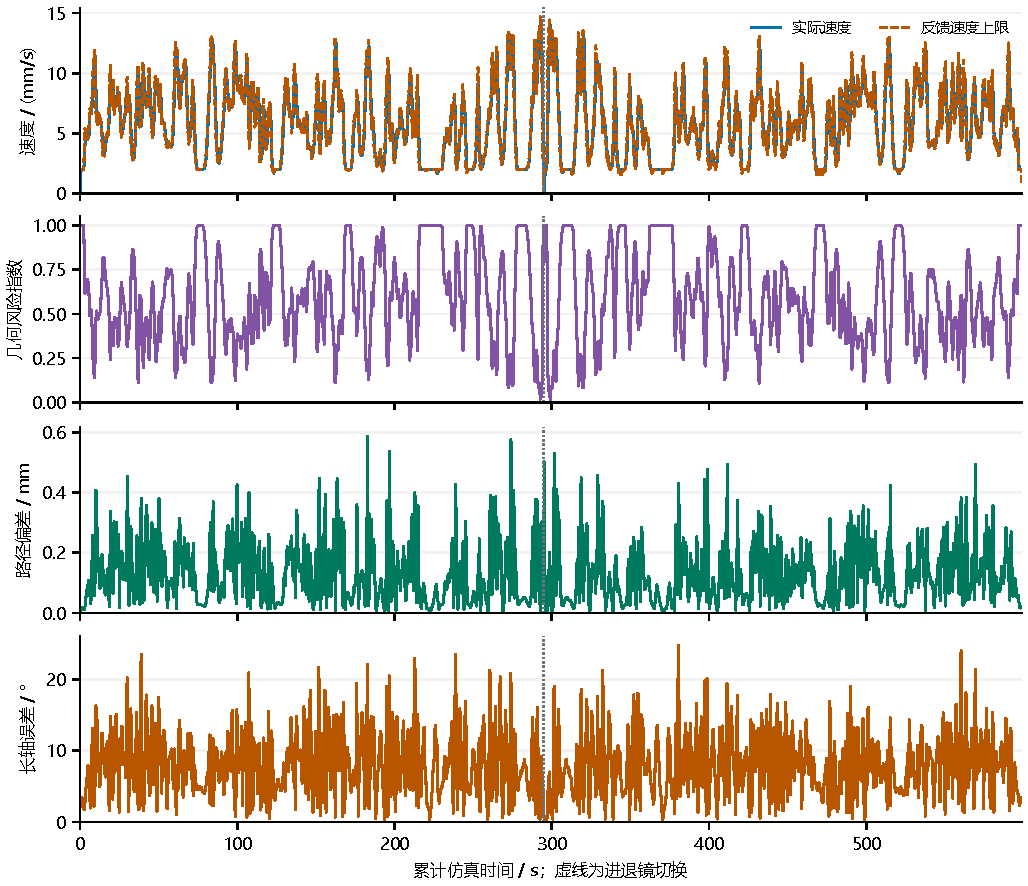
\includegraphics[width=\linewidth]{fig03_motion.pdf}
\caption{全程运动与导航状态。虚线分隔进镜和退镜；上限会随风险、曲率、净空和相机状态改变。实际速度由磁力积分得出，但受速度包络反馈调节。路径偏差按保存样本所用参考计算，不是组织接触距离。}\label{fig:motion}
\end{figure}

\subsection{八路电流、总场与推进力}
八路电流随全程姿态和推力需求改变，见图\ref{fig:currents}。初始电流约为
\begin{equation}
\begin{split}
(I_1,I_2,I_3,I_4)&=(2.573,0.946,4.275,0.206)\unit A,\\
(I_5,I_6,I_7,I_8)&=(0.981,-2.634,-1.348,-1.821)\unit A.
\end{split}
\end{equation}
电流符号表示源磁矩沿轴线或反轴线，不是正负两类物理磁铁。

保存样本中，磁力幅值约4.16--6.20毫牛顿，梯度Frobenius范数约0.197--0.321特斯拉每米；总场三个分量持续变化而幅值几乎恒定，见图\ref{fig:field}。当前同一模型下的场跟踪残差最大约$1.12\times10^{-16}\unit T$，力跟踪残差约$4.25\times10^{-17}\unit N$，只是代数一致性和本参数组合可达的表现，\textbf{不是线圈场实测误差}。同模型动力学重建一致性也不能替代独立数值模型或台架验证。
\begin{figure}[p]
\centering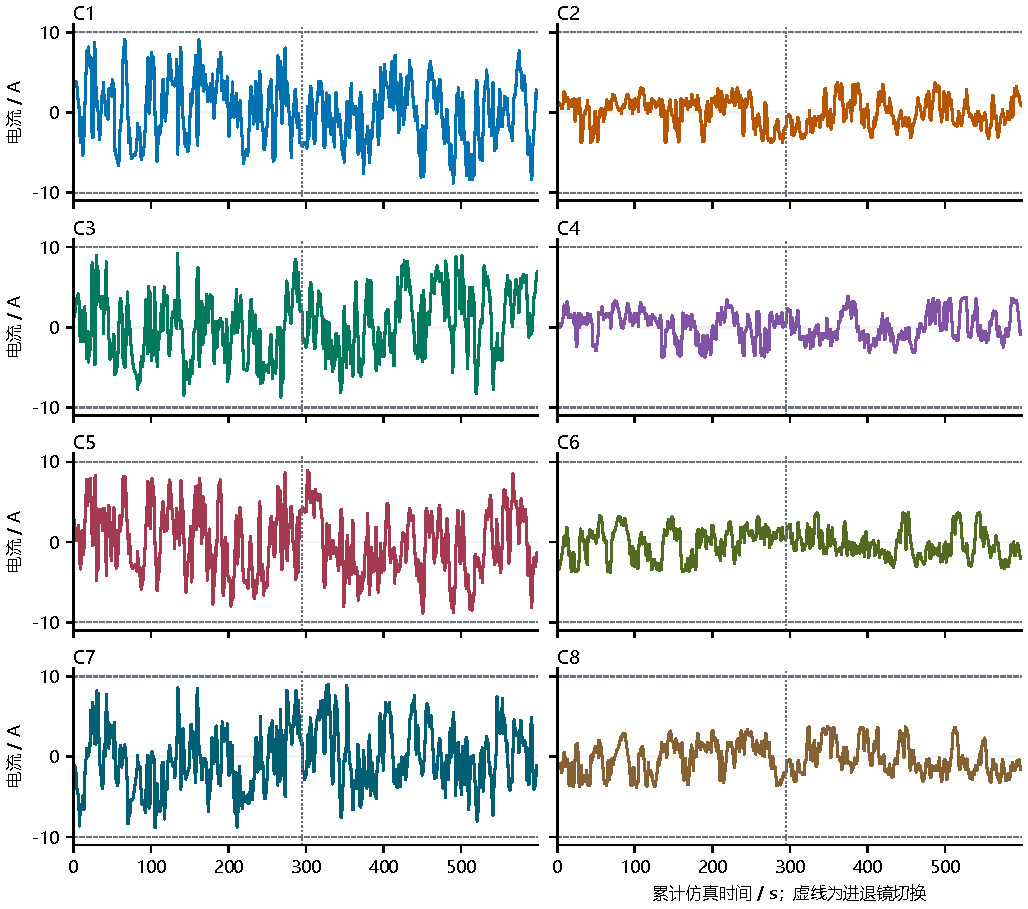
\includegraphics[width=\linewidth]{fig04_currents.pdf}
\caption{C1--C8的电流回放。各子图共享纵轴，灰色横虚线为$\pm10$安培，竖虚线为阶段切换。电流变化由理想执行器直接实现，未加入电流斜率、感应电压或热约束。}\label{fig:currents}
\end{figure}
\begin{figure}[p]
\centering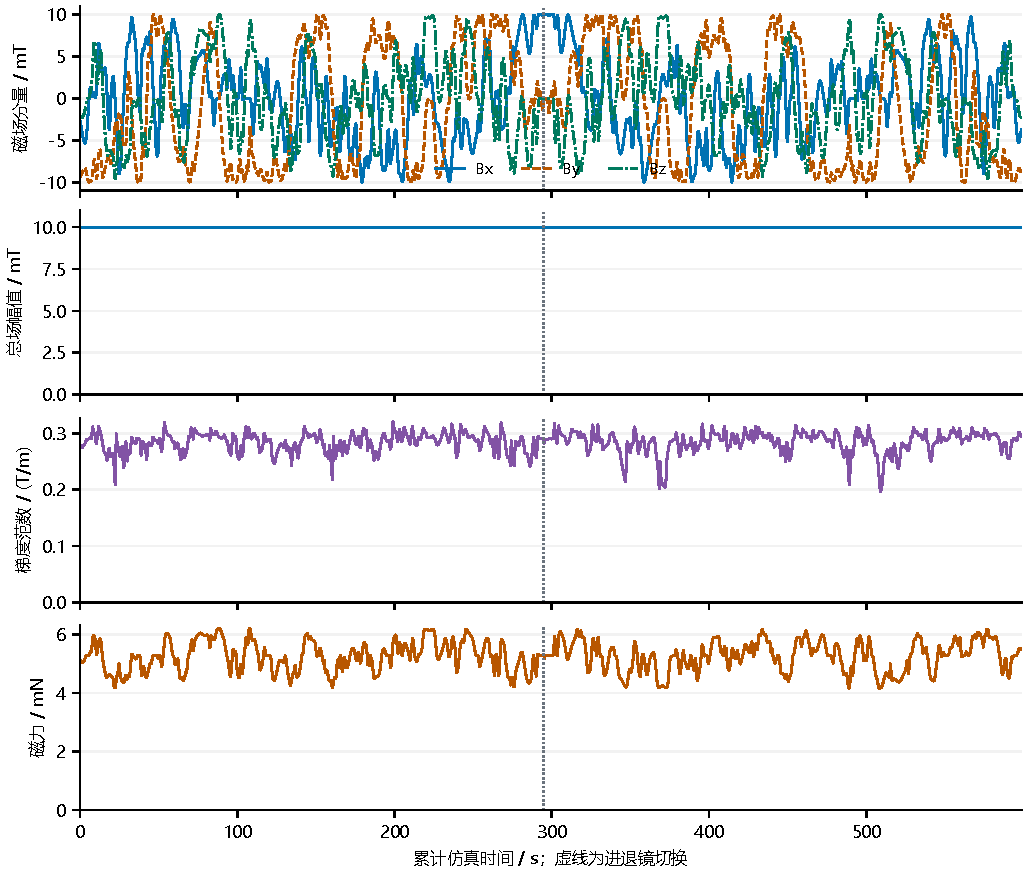
\includegraphics[width=\linewidth]{fig05_field_force.pdf}
\caption{胶囊当前位置的场分量、总场幅值、梯度范数与磁力。总场图从零起轴，避免将$10^{-8}$毫特斯拉量级的幅值变化夸大为控制效果。场强接近恒定与推进力变化可以同时成立。}\label{fig:field}
\end{figure}

\FloatBarrier
\subsection{退镜搜索、相机运动与去重覆盖}
退镜执行760次决策，每次搜索243--381个方向。现有记录中，预测fallback与实际检查到的云台越限样本均为0。其含义是本次离散检查通过，不是所有连续时间状态、未知扰动或其他病例均安全。云台运动和面积曲线见图\ref{fig:coverage}。

\begin{table}[htbp]
\centering\caption{统一几何、遮挡、像素及观察时长门槛下的面积结果。}
\begin{tabularx}{\linewidth}{Xrr}
\toprule 面积类别 & 面积 / mm$^2$ & 占总内壁面积 / \%\\\midrule
进镜已有效观察 & 165529.21 & 67.1743\\
退镜去重新增 & 31240.72 & 12.6780\\
最终去重合计 & 196769.93 & 79.8523\\
仍未达标 & 49647.54 & 20.1477\\
评价内壁总面积 & 246417.47 & 100.0000\\\bottomrule
\end{tabularx}
\end{table}

退镜带来12.6780个百分点的新增覆盖，或相对进镜已覆盖面积增加18.8732\%；两种分母不同，不应混写为“提升12.68\%”。当前没有在同一新磁驱动轨迹上重做固定相机、旧37方向或无预测版本的对照，因此该新增量不能单独归因于密集搜索或短时预测优于所有基线，也不能声称统计显著。
\begin{figure}[p]
\centering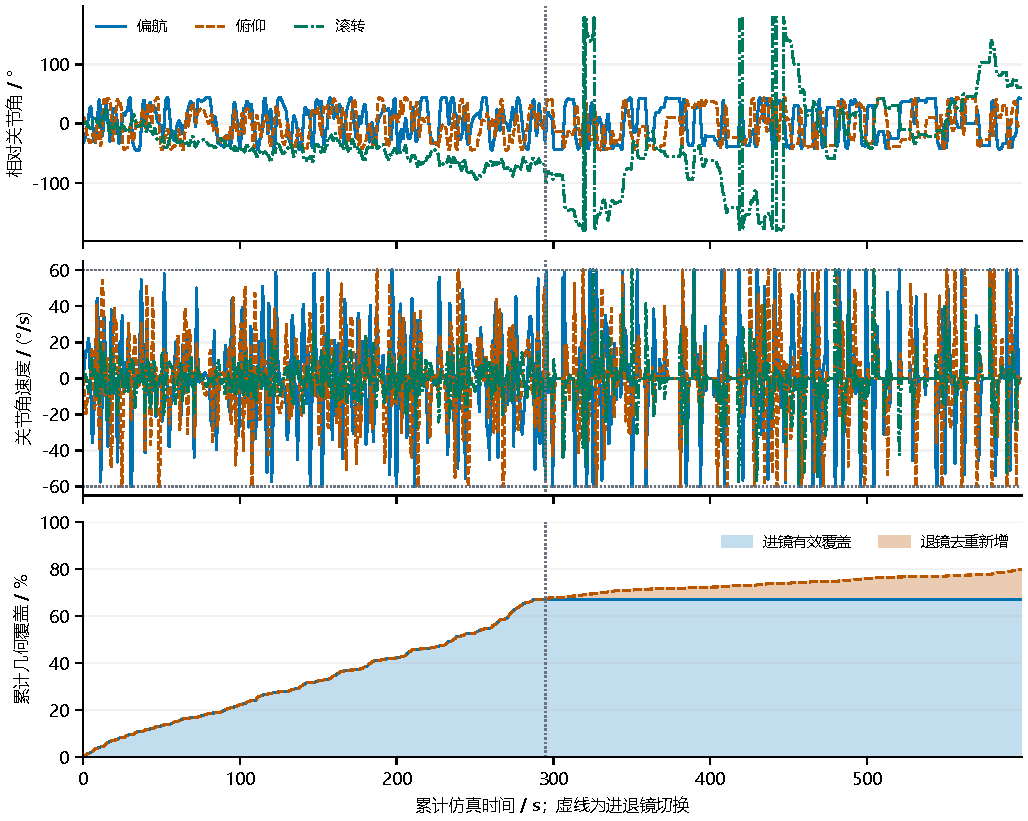
\includegraphics[width=\linewidth]{fig06_camera_coverage.pdf}
\caption{相对机身的云台关节角、关节角速度及累计几何有效覆盖。蓝色实线为进镜集合，橙色虚线为两阶段合计，橙色填充为去重新增。纵轴从0至100\%，避免夸大覆盖变化。滚转采用包角表示，跨界不代表瞬时物理转动；应结合速度图解读。}\label{fig:coverage}
\end{figure}

\FloatBarrier
\subsection{规划耗时与显示帧率不能混同}
本次退镜规划的平均耗时为260.6毫秒、P95为325.9毫秒、记录最大值为376.2毫秒。虽然它们低于400毫秒决策周期，该记录仅对应一次离线运行，不能替代最坏执行时间或传感、通信、调度的在线测量。可见性渲染使用本机NVIDIA RTX 5060 Laptop GPU；电流分配与动力学仍为当前CPU数值实现，没有使用Mworks有限元求解或训练神经网络。

桌面程序采用原生Qt与OpenGL回放已生成轨迹。播放顺滑反映插值和渲染性能，并不说明每一帧都完成磁场优化；规划耗时、动力学积分耗时和播放帧率应分别报告。

\section{潜在临床意义、研究定位与后续验证}
\subsection{褶皱后方盲区：仍需应对的临床难点}
结肠皱襞会使其背向当前镜头的一侧黏膜被前景组织遮挡；镜头向前通过，并不等于褶皱后方已经暴露。这是结肠镜检查中较难完全消除的黏膜暴露问题，病灶若位于未显露表面，即使后续图像识别准确，也可能没有可供判读的影像。Leufkens等在随机、多中心串联结肠镜研究中指出，传统结肠镜可能漏掉位于皱襞后方或弯曲内侧的腺瘤，并评价了增加反向视角的观察装置\cite{leufkens2011}。Gralnek等的多中心随机串联研究则比较了标准前视结肠镜与扩展视场系统，研究通过扩大观察范围减少漏检的可能性\cite{gralnek2014}。这些原始研究支持将黏膜暴露和几何盲区作为研究目标，但不代表某一种装置或控制方法已彻底解决该问题。

\textbf{延长停留或提高图像分辨率，不能单独消除同一视线上的完全几何遮挡。}需要通过视点移动、镜头转向或额外观察方向等方式改变可见关系；真实检查还涉及充气、体位和组织形变等操作，本项目尚未对这些过程建模。在固定中心线路线与受限云台下，单纯转动镜头也未必能看到所有背侧表面，因此本方法不承诺消除全部褶皱盲区。

本文退镜搜索的作用，是在现有运动与视角约束内，利用式\eqref{eq:depth_buffer}--\eqref{eq:visible_pixels}区分遮挡后的实际可见面片，优先补充尚未达标区域的观察；这是对临床暴露难题的几何代理任务。当前79.85\%为全网格面片级几何覆盖，既不是褶皱背面专门覆盖率，也不是临床病灶检出率。后续应在有明确褶皱背侧标注和已知病灶位置的体模中，分别报告背侧暴露率、病灶可见率及医生判读结果，检验覆盖增益能否转化为检查获益。

\subsection{对临床研究可能有用的方面}
该方法的第一项潜在价值，是把“走得到”和“看得到”作为相互约束的任务，而不只追求机器人沿中心线运动。前瞻相机用于进镜过程的方向观察，退镜主动关注未达标区域，减速反馈为镜头跟随留出更多时间。若未来在真实定位、图像质量和接触约束下仍有效，可能为减少重复无效观察、定位观察不足区域和记录检查过程提供技术基础。

第二项价值，是从任意理想场需求走向带磁源结构与电流界的可实现性评估。它使“需要什么力/转矩”和“外部装置实际能提供什么”之间出现可计算接口，有利于后续比较线圈布局、驱动裕量及不同机械方案。但当前每安培等效磁矩较强且没有热设计，故不应据此直接选型实物线圈或宣称已完成现实迁移。

第三项价值，是将覆盖定义和约束留有可追溯记录。对于后续体模或临床前实验，可将几何观察集合与真实图像质量、病灶位置、医生判读及接触力联系起来。已有磁内镜研究说明机器人、视觉与控制的结合具有转化研究基础\cite{martin2020}，但本文没有患者实验，不能声称降低疼痛、减少并发症、提高腺瘤检出率或改善患者结局。

\subsection{创新定位应当如何表述}
可以作为候选研究贡献的是：在既定结肠路线中，将受限多磁源驱动、前瞻进镜、近最优平滑退镜补拍与覆盖记忆驱动的协调纳入同一动力学流程，并清楚报告运动、观察及计算约束。是否构成可发表创新仍需同任务、同预算的对照和跨病例验证。八线圈、PD、磁场优先或滑窗搜索各自已有技术背景，不能单独被宣称为首创。

当前实现\textbf{不包含CNN、PINN或FNO}。上游分割即使使用学习模型，也不能据此把本稿的电流分配称为神经网络控制。Raissi等提出的PINN\cite{raissi2019}及Li等提出的FNO\cite{li2021}可作为未来高保真磁场代理模型的候选，而非本次已完成的组成部分。

若将来用有限元或实测线圈替换点偶极源，可考虑学习
\begin{equation}
(\vect x,\vect p_i,\vect a_i,\vect I,\text{材料/几何})\longmapsto(\vect B,G),
\label{eq:future_surrogate}
\end{equation}
并在无源均匀区域加入式\eqref{eq:maxwell}的物理残差，再把代理输出接入同一力/转矩接口。学习逆分配时则还需满足电流、温升和可达性约束，并配置高保真回退。由于当前解析点偶极叠加本身很便宜，仅为它训练大型网络未必加速；必须报告精度、梯度误差、推理时延和闭环轨迹误差，而不是只报告磁场均方误差。式\eqref{eq:future_surrogate}为研究方向，不是本文已实现公式。

\subsection{从方法仿真到可信实物研究的顺序}
优先补齐真实线圈尺寸、绕组、磁芯、驱动器与热约束，并在关注工作空间标定$\vect B$和$G$；随后验证单点力/转矩能力、阵列碰撞和机械臂运动限制。建立位置/姿态估计及实测电流反馈后，再进行带真实摩擦的管道或结肠体模实验，不能跳过接触与安全问题直接推向人体。

算法层面应在同一几何、路径与时间预算下比较：理想磁场与磁源约束；固定相机、旧37方向、密集单步搜索和密集短时预测；无相机减速与只减速。还应做电流上限、磁矩、质量、摩擦、体位、源距离、定位噪声和延迟的敏感性实验，并记录不成功案例。核心指标包括路线完成率、接触/碰撞代理、峰值电流与热裕量、长轴误差、图像质量、去重覆盖、最差规划耗时和故障恢复。

真实检查质量最终仍需病灶真值和临床判读评价。本文提出的是可复核的方法链条与单例证据，不是医疗器械安全认证、临床方案或人体操作建议。

\section{结论}
在已知静态结肠几何、理想滑动阻力、准确状态反馈和八等效点磁源假设下，当前实现完成了从磁力需求到受限电流、实际磁源输出、刚体运动、相机执行及去重观察面积的完整数值流程。clon001往返成功和退镜新增覆盖支持该组参数下的仿真可行性。局部PD稳定性可解释纠偏和云台执行的合理性，但不能替代整体非线性系统的安全与稳定性证明。方法下一步的重点应是高保真磁源标定、接触和传感闭环，以及有控制条件的跨病例与体模验证。
\clearpage\appendix
\section{参数总表及其来源层级}
\small
\begin{longtable}{>{\raggedright\arraybackslash}p{.31\linewidth}>{\raggedright\arraybackslash}p{.27\linewidth}>{\raggedright\arraybackslash}p{.33\linewidth}}
\caption{当前有效参数。工程初值表示已在本次实现使用，但未优化或实测；继承值不自动等于当前执行值。}\label{tab:parameters}\\
\toprule 参数 & 当前数值 & 来源与解释\\\midrule\endfirsthead
\multicolumn{3}{l}{表\thetable\ （续）}\\\toprule 参数 & 当前数值 & 来源与解释\\\midrule\endhead
胶囊长度、直径 & 12、6 mm & 工程尺寸假设\\
体积缩放比$\eta$ & 0.1022485 & 式\eqref{eq:scaling}\\
质量$M$ & 0.527602 g & 按体积继承缩放，非称重\\
磁矩幅值$m_0$ & 0.0258689 A m$^2$ & 按体积缩放，非标定\\
椭球惯量$J_{xx}$ & $2.1843\times10^{-9}$ kg m$^2$ & 均匀椭球近似\\
椭球惯量$J_{yy}=J_{zz}$ & $5.7456\times10^{-9}$ kg m$^2$ & 均匀椭球近似\\
重力 & $(0,0,-9.81)$ m/s$^2$ & 世界系固定向下\\
摩擦系数$\mu$ & 0.2 & 沿用理想阻力参数\\
平滑速度$v_\epsilon$ & 0.5 mm/s & 无静摩擦粘滞\\
等效法向负载 & $M\norm{\vect g}\approx5.176$ mN & 不是壁面接触力\\
横向$k_p,k_d$ & 16 s$^{-2}$、8 s$^{-1}$ & 工程PD初值\\
长轴$k_a,k_\omega$ & 25 s$^{-2}$、10 s$^{-1}$ & 仅指向控制\\
纵向响应$T_v$ & 0.25 s & 上限趋近调节\\
推进、制动加速度界 & 8、8 mm/s$^2$ & 指令界，不是总加速度硬保证\\
侧向加速度指令界 & 40 mm/s$^2$ & 未建模接触时的工程界\\
风险速度参数 & 2、15 mm/s；指数1.4 & 式\eqref{eq:speed_limits}\\
净空速度参数 & 胶囊半径3、参考半径16 mm & 净空比例裁剪0.15至1\\
上游风险权重 & 1、1.5、0.8、1、0.6 & 贴壁/狭窄/曲率/敏感/运动代理\\
风险半径尺度 & 5、3、7 mm & 上游工程阈值，非临床界\\
曲率、转向尺度 & 0.12 mm$^{-1}$、0.35 rad & 上游归一化尺度\\
局部弧长投影窗 & $\pm25$ mm & 减少跨肠袢误匹配\\
相机减速系数$D$ & 1至1.25 & 上限最多降低20\%\\
减速触发尺度 & 误差15度、速度50度/s & 增益分母80、120\\
磁偏置场$B_0$ & 10 mT & 生成器覆写旧输入15 mT\\
源数量 & 8 & 相对布局固定\\
每安培等效磁矩$k_M$ & 20 A m$^2$/A & 未由绕组/铁芯/热约束核验\\
每路电流界 & $\pm10$ A & 无电流变化率界\\
源方位角 & 0至315度，间隔45度 & C1至C8依次编号\\
源极角 & 35度、60度交替 & 相对世界$+Z$\\
源到锚点距离 & 160、130 mm交替 & 不是物理线圈半径\\
阵列移动速度界 & 0.20 m/s & 整体移动，无机械臂关节模型\\
锚点目标更新 & 0.2 s & 间隔内位置线性插值\\
电流分配执行 & 每次动力学右端计算 & 含RK4子阶段，理想即时执行\\
SVD秩判断 & 相对最大奇异值$10^{-12}$ & 数值阈值\\
SLSQP力分配 & 最多80次迭代；容差$10^{-12}$ & 不等于全局可行性证书\\
动力学积分 & RK4，0.02 s & 不是继承配置字段DOP853\\
状态保存/最终覆盖 & 约0.1 s，保留结束点 & 不是旧说明中的进镜0.4 s\\
阶段超时界 & 700 s & 每阶段生成上限\\
终点弧长/距离容差 & 0.15 mm、1 mm & 同时满足，无位置吸附\\
起始机身扰动 & 世界轴角$[0,0,3]$度 & 实际起点位置无0.5 mm偏移\\
光心安装偏移 & 5.8 mm & 沿机身$+X$\\
垂直视场、宽高比 & 60度、4:3 & 水平视场由比例导出\\
云台光轴锥、机械角界 & 45度；偏航/俯仰$\pm89$度 & 光轴约束非视场角点约束\\
云台PD增益 & 12 s$^{-2}$、6 s$^{-1}$ & 角度使用度\\
云台速度、加速度界 & 60度/s、150度/s$^2$ & 每轴独立检查\\
云台积分子步 & 至多0.01 s & 角限附加制动\\
前瞻公式系数 & 12、1.8、25、0.8 & 毫米/秒单位体系，式\eqref{eq:lookahead}\\
前瞻距离、净空上界 & 5至45 mm；$6+2c$ & 实际使用保存目标而非重算\\
前瞻方向迟滞门槛 & 0.50、0.45 & 首次/已有目标\\
前瞻变化率、候选间隔 & 10 mm/s、3 mm & 目标生成器设定\\
退镜决策、预测期 & 0.4 s、1.2 s & 预测不强制机器人运动\\
粗搜、细搜角步长 & 10度、2度 & 不是固定37方向\\
细化区域、方向候选 & 3个、最多6个 & 另加实际角和旧目标\\
收益容差 & 最佳可行候选收益的95\% & 候选集内近最优\\
平滑代价权重 & 0.05、1、0.1 & 速度/加速度/角加加速度\\
角加加速度归一化 & 1500度/s$^3$ & 代价尺度，非硬件界\\
深度图集 & 六面，每面192$\times$192 & 粗筛遮挡集合\\
最终面片ID图 & 160$\times$120 & 无光照、深度测试\\
合格距离、入射角 & 2至80 mm、不超过75度 & 面片中心近似\\
最小面片像素 & 2 & 几何图像门槛\\
累计观察、重启间隙 & 0.4 s、0.8 s & 相邻两端均可见才计时\\
评价面片数 & 33696 & 单一内表面网格\\
真实绕组/电感/热参数 & 尚无 & 不能从示意圆环推断\\
定位、图像、接触反馈 & 尚无 & 当前使用仿真真值\\
\bottomrule\end{longtable}\normalsize

\clearpage
\section{核心符号与实现对应}
\begin{longtable}{>{\raggedright\arraybackslash}p{.20\linewidth}>{\raggedright\arraybackslash}p{.30\linewidth}>{\raggedright\arraybackslash}p{.41\linewidth}}
\toprule 符号 & 含义与单位 & 当前实现对应\\\midrule\endfirsthead
\toprule 符号 & 含义与单位 & 当前实现对应\\\midrule\endhead
$\vect p,\vect v,\vect q,\vect\omega_b$ & 位移、速度、四元数、机身角速度 & 13维动力学状态\\
$M,\vect m,J$ & 质量、胶囊磁矩、惯量 & \code{coil_simulation/model.py}\\
$\vect F_{\rm fr}$ & 理想平滑滑动阻力，N & \code{model.resistance}\\
$\sigma,\vect r,\vect t$ & 阶段弧长、路线、单位切向 & \code{path_guidance.SpatialRoute}\\
$r,c,\kappa$ & 几何风险、净空、曲率 & 保存的\code{source}数组\\
$D,v_{\rm cap}$ & 相机膨胀系数、速度上限 & \code{effective_speed_cap}\\
$\vect F_c,\vect\tau_c$ & 期望磁力、转矩 & \code{magnetic_path_demand}\\
$\vect B_d,G_{\rm ideal}$ & 理想目标场、对照梯度 & \code{inverse_field/minimum_gradient}\\
$\vect h,\vect o_i,\vect a_i$ & 阵列锚点、源偏移与轴线 & \code{simulation.py}及\code{redundant_actuator.py}\\
$\vect M_i,I_i$ & 源磁矩与电流 & \code{coil_physics.py}\\
$A_B,A_F,Z$ & 场映射、力映射、场零空间 & \code{allocate_field_priority}\\
$\vect p_c,R_c,\vect\theta$ & 光心、相机旋转、ZYX角 & \code{CameraPolicy}及\code{controller.py}\\
$\pi,\Delta A,J(\pi)$ & 镜头方案、收益、平滑代价 & \code{planning.py}\\
$A_i,V_i,d_i$ & 面积、合格可见性、累计时长 & \code{visibility.py/coverage.py}\\
$\mathcal C_{\rm in},\mathcal C_{\rm out}$ & 进退镜合格观察集合 & \code{evaluate_coverage}\\
\bottomrule\end{longtable}

\section{证据文件、复现与不可沿用的旧字段}
本稿以\code{navigate software pt2}的当前有效源码、\code{数据/clon001}及\code{文档/八线圈仿真结果.json}为基础。配套目录提供图表原始CSV、绘图脚本、参考文献信息核验、源码与数据SHA-256清单，以及版式检查报告。曲线和表中数值都可回溯到这些文件。没有修改软件控制代码或重新调参来提高本稿结果。

应特别避免引用以下继承字段作为当前执行事实：输入配置的15毫特斯拉偏置已被生成器覆写为10毫特斯拉；原配置的DOP853不是当前RK4；旧相机说明的334.129秒退镜、0.4秒进镜评价及未改动进镜覆盖等表述，不适用于本次磁源与轨迹重算；注册表继承的样本数也不应替代实际5987行。参数判断优先顺序是当前执行入口、有效输出数据、对应生成报告，最后才是沿用的说明文字。

\subsection*{研究诚信与AI辅助说明}
本稿由AI辅助核对代码、整理推导、重绘图表并撰写，所有数值取自既有仿真或本文直接描述性统计。未编造患者、实验批次、统计显著性、硬件测量或临床结果。正式投稿前仍需作者逐式复核、补充研究设计与对照，并按目标期刊要求披露AI使用及确认署名责任。

\clearpage
\addcontentsline{toc}{section}{参考文献}
\begin{thebibliography}{9}
\bibitem{kummer2010}
Kummer M P, Abbott J J, Kratochvil B E, Borer R, Sengul A, Nelson B J.
OctoMag: An Electromagnetic System for 5-DOF Wireless Micromanipulation.
\textit{IEEE Transactions on Robotics}, 2010, 26(6): 1006--1017.
DOI: \href{https://doi.org/10.1109/TRO.2010.2073030}{10.1109/TRO.2010.2073030}.
\bibitem{cai2025}
Cai M, Qi Z, Cao Y, Wu X, Xu T, Zhang L.
Magnetic Field-Priority Force Control for Automated Manipulation in Large Workspaces With Reconfigurable Electromagnetic Actuation System.
\textit{IEEE Transactions on Industrial Electronics}, 2025, 72(2): 1732--1742.
DOI: \href{https://doi.org/10.1109/TIE.2024.3426055}{10.1109/TIE.2024.3426055}.
\bibitem{martin2020}
Martin J W, Scaglioni B, Norton J C, Subramanian V, Arezzo A, Obstein K L, Valdastri P.
Enabling the future of colonoscopy with intelligent and autonomous magnetic manipulation.
\textit{Nature Machine Intelligence}, 2020, 2: 595--606.
DOI: \href{https://doi.org/10.1038/s42256-020-00231-9}{10.1038/s42256-020-00231-9}.
\bibitem{raissi2019}
Raissi M, Perdikaris P, Karniadakis G E.
Physics-informed neural networks: A deep learning framework for solving forward and inverse problems involving nonlinear partial differential equations.
\textit{Journal of Computational Physics}, 2019, 378: 686--707.
DOI: \href{https://doi.org/10.1016/j.jcp.2018.10.045}{10.1016/j.jcp.2018.10.045}.
\bibitem{li2021}
Li Z, Kovachki N, Azizzadenesheli K, et al.
Fourier Neural Operator for Parametric Partial Differential Equations.
\textit{International Conference on Learning Representations}, 2021.
Preprint: \href{https://arxiv.org/abs/2010.08895}{arXiv:2010.08895}.
\bibitem{leufkens2011}
Leufkens A M, DeMarco D C, Rastogi A, et al.
Effect of a retrograde-viewing device on adenoma detection rate during colonoscopy: the TERRACE study.
\textit{Gastrointestinal Endoscopy}, 2011, 73(3): 480--489.
DOI: \href{https://doi.org/10.1016/j.gie.2010.09.004}{10.1016/j.gie.2010.09.004}.
\bibitem{gralnek2014}
Gralnek I M, Siersema P D, Halpern Z, et al.
Standard forward-viewing colonoscopy versus full-spectrum endoscopy: an international, multicentre, randomised, tandem colonoscopy trial.
\textit{The Lancet Oncology}, 2014, 15(3): 353--360.
DOI: \href{https://doi.org/10.1016/S1470-2045(14)70020-8}{10.1016/S1470-2045(14)70020-8}.
\end{thebibliography}
\end{document}
